\subsection{Inserimento dati climatici per una città}
Ora che il centro di monitoraggio è stato creato, è possibile inserire i dati climatici per le città associate ad esso.\\ 

\begin{figure}[H]
    \centering
    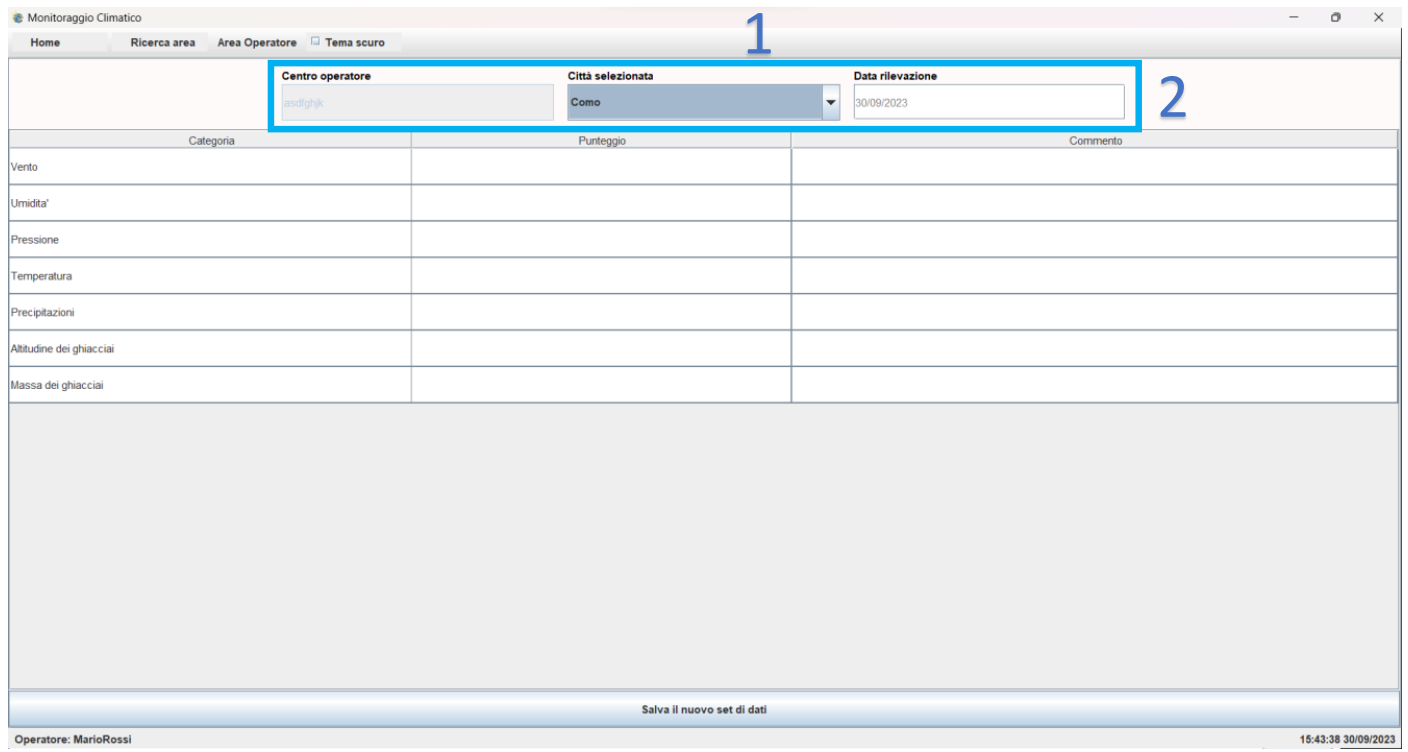
\includegraphics[width=1\textwidth]{../../img/schermata_inserimento_dati.png}
    \caption{Schermata Inserimento dati}
\end{figure}

Nel campo [1] è possibile scegliere per quale città si vogliono inserire i dati climatici, mentre nel campo [2] è possibile scegliere per quale data
si vogliono inserire i dati.
Se non viene modificata la data, verrà inserita la data corrente.\\

Nella tabella sottostante, nella colonna \emph{Punteggio} è possibile inserire il punteggio relativo al parametro climatico in un range da 1 a 5.
Per sapere la suddivisione in fasce dei punteggi, fare riferimento alla sezione \ref{sec:legenda_punteggi} del presente manuale
oppure cliccare sulla categoria desiderata per visualizzare la relativa legenda.\\

\begin{figure}[H]
    \centering
    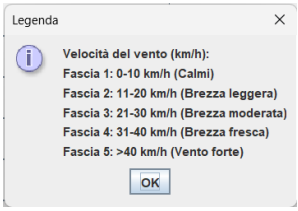
\includegraphics[width=0.7\textwidth]{../../img/esempio_legenda.png}
    \caption{Esempio di legenda}
\end{figure}

Per poter salvare i dati nel sistema, bisogna obbligatoriamente inserire almeno un punteggio. Inoltre, nella colonna \emph{Commento} è possibile
inserire un commento relativo al punteggio inserito, con un limite di 256 caratteri.
Se vengono superati, verrà visualizzato un messaggio di errore e non si potranno salvare i dati a meno che i commenti non rispettino il limite.

\begin{figure}[H]
    \centering
    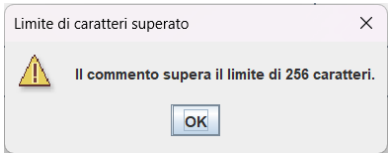
\includegraphics[width=0.7\textwidth]{../../img/avviso_limite_caratteri.png}
    \caption{Avviso limite caratteri}
\end{figure}

Per salvare correttamente i dati premere \emph{Invio} prima di cliccare il pulsante \emph{Salva il nuovo set di dati}.
Una volta salvati i dati, questi potranno essere visuallizati in \ref{sec:dati_città}.\\